% !TEX program = xelatex
% Elsevier elsarticle 版(目标期刊:Mechanical Systems and Signal Processing)。
% 由 tools/to_elsarticle.py 从 IEEEtran 版 manuscript.tex 机械转换而来 —— 正文逐字一致,
% 改内容请改 IEEEtran 版再重跑转换,不要只改这一份。
\documentclass[preprint,12pt]{elsarticle}

\usepackage{amsmath,amssymb}
\usepackage{booktabs}
\usepackage{graphicx}
\usepackage{array}
\usepackage{multirow}
\usepackage{url}
% hyperref 必须排在 orcidlink 之前:orcidlink 内部会加载 hyperref,
% 若先加载 orcidlink,后面再 \usepackage[...]{hyperref} 会报 "Option clash"。
\usepackage[colorlinks=true,allcolors=blue]{hyperref}
\usepackage{orcidlink}

\newcommand{\ml}[1]{\textsc{#1}}

% elsarticle 的 \paragraph 是行内小标题,长标题后面紧跟正文时不给断行机会,
% 会留下 10~22pt 的 Overfull。放开一点点伸缩量即可消掉(纯排版,不改内容)。
\setlength{\emergencystretch}{2em}

\begin{document}

\begin{frontmatter}

\title{Why Simulation-Based Sample Supplementation Fails in Cross-Domain Bearing
Fault Diagnosis: The Recording-Fingerprint Effect and an Evaluation Protocol
That Reveals It}

% 作者信息(2026-10-06 由作者提供)。
% 注意:TeX Live 2026 的 elsarticle.cls 里**完全没有** orcid 支持
% (grep orcid elsarticle.cls 返回 0 处),所以 `\author[1]{Name}[orcid=...]` 那种写法
% 不会被解析,会原样排进 PDF(实测确实如此)。改用已安装的 orcidlink 包
% (包已在导言区加载 —— 它是 \usepackage,放在正文里会报 "Can be used only in preamble")。

\author[1]{Fangyu Zhang\,\orcidlink{0009-0009-7352-1484}\corref{cor1}}
\ead{fyzhang9925@mails.jlu.edu.cn}
\author[2]{Julong He\,\orcidlink{0009-0003-0143-7204}}
\ead{u202541560@xs.ustb.edu.cn}
\cortext[cor1]{Corresponding author.}
\affiliation[1]{organization={College of Mechanical and Aerospace Engineering,
                            Jilin University},
                city={Changchun},
                postcode={130025},
                country={China}}
\affiliation[2]{organization={National College for Excellent Engineers,
                            University of Science and Technology Beijing},
                city={Beijing},
                postcode={100083},
                country={China}}

\begin{abstract}
Physics-based simulation, notably ``digital twin'' generators, is a
popular source of synthetic fault samples for cross-domain bearing fault
diagnosis when labeled target data are scarce. On the standard CWRU 12\,kHz
drive-end benchmark it is \emph{structurally} unable to supply
class information. Every ``fault type $\times$ load'' cell is a \emph{single
recording}, and the class-conditional magnitude spectrum is a stable property
of it: a class's spectral envelope recurs across the four loads at cosine
$0.944$, yet is not predictable from fault physics, since a source-domain
envelope transfers to the target at $0.924$ while one estimated from five
labeled \emph{target} samples reaches $0.995$. Class identity is thus a
per-bearing \emph{recording fingerprint}. A calibrated McFadden--Smith twin
produces nine classes with near-identical
spectra and, trained on twin data alone, reaches macro-F1 $0.123$ (chance
$0.10$). Its few-shot protocol compounds this: support and test
windows share the fingerprint, so cross-recording evaluation lowers reported
macro-F1 by $0.15$--$0.19$ (up to $0.31$) and equalizes
augmentation-based methods with the trivial baseline. Coloring white noise with
the target envelope is the most robust augmentation when the target recording
is atypical; adding a physical impulse train degrades fidelity and
accuracy. On Paderborn, where several bearings share each class, class-mean
spectra remain indistinguishable (cosine $1.000$) although classes are defined
by damage location; there same-recording optimism of $+0.340$ splits
into session ($+0.182$) and specimen ($+0.158$) terms. The advantage of
fingerprint calibration over raw physics inverts between the benchmarks.
\end{abstract}

\begin{keyword}
bearing fault diagnosis \sep
benchmark evaluation \sep
cross-domain transfer \sep
digital
twin \sep
few-shot learning \sep
simulation-based data augmentation \sep
spectral
fingerprint
\end{keyword}

\end{frontmatter}

\section{Introduction}
\label{sec:intro}

Deep models for bearing fault diagnosis are notoriously fragile under domain
shift, and the scarcity of labeled data on a newly commissioned machine makes
transfer learning unavoidable. Two families of remedies dominate the
literature: (i) unsupervised domain adaptation, typically adversarial
\cite{ganin2016dann} or moment-matching \cite{sun2016coral}, and (ii) the
generation of additional labeled samples
for the target operating condition, either by physics-based simulation
\cite{ming2026physics, xiao2026sim2real, liu2024twin} or by generative models
\cite{shao2019gan}.

The simulation route is attractive because a physical model is, in principle,
transferable \cite{karniadakis2021piml, tao2019dt}: bearing characteristic
frequencies scale with shaft speed, so a
model of a spalled outer race at $1797$\,rpm can be re-instantiated at
$1730$\,rpm without any new data. Many recent papers report that augmenting
training with simulated faults improves cross-domain accuracy
\cite{liu2024twin, xu2024dt, zhang2023dt, kumar2024dt, ming2026physics,
xiao2026sim2real}.

This paper asks a prior question that the field has largely skipped:
\emph{what class-related information can a physical simulator actually
supply on the benchmarks we use to test it?} We answer it for the most widely
used benchmark, the CWRU 12\,kHz drive-end dataset, and the answer is
uncomfortable: on this benchmark the simulator supplies essentially nothing,
for a structural reason, and the experimental protocol used to evaluate such
methods is itself inflating results.

\subsection{Contributions}
\begin{itemize}
\item \textbf{C1 (diagnosis).} A physically calibrated twin remains
$99.99\%$ separable from real data under a domain discriminator, and a
classifier trained only on twin data transfers to the real target domain at
macro-F1 $=0.123$, i.e.\ chance for ten classes (Section~\ref{sec:diag1}).
\item \textbf{C2 (root cause).} Class identity in CWRU is dominated by a
\emph{recording fingerprint}. Per-class spectral envelopes are stable across
loads (cosine $0.944$ averaged over all load pairs), but the source-domain
envelope predicts the target-domain envelope only to $0.924$. The twin
reproduces neither (Section~\ref{sec:diag2}).
\item \textbf{C3 (protocol).} The few-shot evaluation protocol draws support
and test windows from the same recording, so both share the fingerprint. Under
a cross-recording protocol the reported macro-F1 drops by $0.15$--$0.19$
(average over four support domains; up to $0.31$), and augmentation-based
methods become indistinguishable from training on the labeled support set alone
(Section~\ref{sec:protocol}). We recommend this control for future work.
\item \textbf{C4 (constructive).} Estimating the per-class spectral envelope
from $k$ labeled target samples is accurate ($0.995$ cosine at $k=5$), and
coloring white noise with it is the most robust augmentation when the target
recording is atypical. Adding a physical impulse train on top of it
\emph{degrades} both domain fidelity and accuracy, consistently across
settings (Sections~\ref{sec:method} and~\ref{sec:results}).
\item \textbf{C5 (side finding).} Load~3 of CWRU is an outlier operating
condition: label-free transfer among loads 0--2 exceeds $0.98$, while any
transfer involving load~3 falls to $0.64$--$0.76$. Conclusions drawn from the
popular S0$\rightarrow$S3 direction alone do not generalize
(Section~\ref{sec:protocol}).
\item \textbf{C6 (cross-benchmark).} On Paderborn, where several independent
bearings share each damage class, class-mean magnitude spectra of healthy,
inner-ring and outer-ring bearings are identical (cosine $1.000$; CWRU:
$0.626$), and remain so after the dominant rig tone is filtered out (margin
$+0.003$). The CWRU class separation is therefore a property of the individual
specimens, not of the classes. Same-recording evaluation is optimistic by
$+0.340$ macro-F1 there; because each Paderborn bearing was measured $20$
times, that optimism can be split by re-evaluating on a different
\emph{recording of the same bearings}, which gives $+0.182$ for the session
and a further $+0.158$ for the change of specimen. A twin whose physics
exactly matches the class definition is still the worst augmentation tried. The
advantage of fingerprint calibration over raw physics inverts between CWRU and
Paderborn in the direction the mechanism predicts, which serves as a positive
control (Section~\ref{sec:paderborn}).
\end{itemize}

\section{Related Work}
\label{sec:related}

\paragraph{Cross-domain and few-shot bearing diagnosis.}
The problem setting we study is standard: a model trained under one operating
condition must be reused under another, and labels are scarce on the target
\cite{lei2020roadmap, zhao2020benchmark}. The dominant response is unsupervised
domain adaptation, usually adversarial, which aligns source and target feature
distributions without target labels \cite{ganin2016dann, wang2018dasurvey,
zhao2021transfer}. A complementary line
attacks label scarcity directly through meta-learning and metric-based few-shot
schemes \cite{wang2020fewshot}, while the backbone architectures themselves are
now well surveyed \cite{jiao2020cnn}. Both are typically evaluated on CWRU or a
handful of sibling benchmarks, and both depend on the support set being
representative of the target test distribution. We show that under the usual
window-level split this assumption is violated in a specific and quantifiable
way.

\paragraph{Simulation and digital-twin sample supplementation.}
Because a physical model transfers by construction, generating labeled fault
samples by simulation is attractive precisely when target labels are missing.
Recent work builds bearing dynamics models and uses the resulting \emph{twin
data} as a labeled source: partial domain adaptation driven by a digital twin
\cite{zhang2023dt}, discriminative graph learning that transfers knowledge from
simulated to real signals \cite{xu2024dt}, multimode collaborative transfer
learning on twin samples \cite{liu2024twin}, and digital-twin-assisted domain
adversarial frameworks for machinery such as centrifugal pumps
\cite{kumar2024dt}. A recurring theme in this literature is the
simulation-to-reality gap, and much of the machinery --- physics-enhanced
translation between simulated and measured signals \cite{ming2026physics},
generative alignment of the two distributions \cite{xiao2026sim2real} --- exists
to close it. The same gap motivates domain randomization in robotics
\cite{tobin2017domain}, where the simulator is deliberately not made faithful
and the burden shifts entirely onto the augmentation distribution.

Our contribution is orthogonal to closing that gap. We ask what
class-discriminative information the simulated data can carry in the first
place, given the structure of the benchmark, and we answer it with a negative
result that no amount of gap-closing can repair: on CWRU the class-conditional
spectrum is a property of the individual recording rather than of the fault, so
a simulator with perfect fidelity to the physics still cannot supply the
contrast that separates the classes.

\paragraph{Surrogate data.}
Our phase-randomization control follows the standard surrogate-data procedure
for testing whether a statistic depends on structure beyond the power spectrum
\cite{theiler1992surrogate, schreiber2000surrogate}. We use it in the reverse
direction from the usual
application: rather than asking whether a signal is nonlinear, we use
phase-randomized surrogates as a deliberately \emph{structure-free} augmentation
baseline, to separate the contribution of the spectral envelope from that of any
temporal structure.

\section{Data, Taxonomy and Protocol}
\label{sec:setup}

\subsection{CWRU and the ten-class taxonomy}
We use the CWRU 12\,kHz drive-end recordings \cite{smith2015cwru}. The
conventional four-class
taxonomy (normal, ball, inner race, outer race) is saturated on cross-load
transfer --- a source-only model reaches $100\%$ accuracy in all twelve
transfer directions --- so we adopt a ten-class taxonomy:
$\{\textsc{Normal}\} \cup \{B,IR,OR\} \times \{0.007'', 0.014'', 0.021''\}$,
using the official files for the four loads $\{0,1,2,3\}$
($1730$--$1797$\,rpm). Windows of $1024$ samples with stride $512$ are
$z$-scored individually.\footnote{Every spectral scalar reported in this paper
is reproduced, from the raw data, by one script released with the code
(\texttt{tools/probe\_spectral\_numbers.py}). We make the point explicitly
because a claim of this paper is that numbers reported in this area do not
always survive re-derivation, and that claim would be worthless if our own did
not.}

\subsection{Few-shot split, and the defect we exploit later}
For a target load, each class is split in time order: the last $40\%$ of
windows form the held-out test set; from the first $60\%$, $k$ windows per
class are drawn (with the seed) as the labeled \emph{support} set, and the rest
form an unlabeled \emph{pool}. Crucially, the support and test windows come
from the \emph{same recording}. Section~\ref{sec:protocol} shows this is not a
detail.

\section{Diagnosis I: What the Twin Supplies}
\label{sec:diag1}

\subsection{The generator}
We implement a McFadden--Smith style impulse-response twin
\cite{randall2011rolling} with SKF 6205-2RS geometry, whose
ball-pass frequencies are computed from the shaft speed. The generator is
calibrated against real CWRU spectra: the resonance range, the resonance
bandwidth per defect size, the background-noise colouring, and the
impulse-to-harmonic power ratio were all fitted so that synthetic
band-energy shares match measured ones. In particular the synthetic peak
envelope spectrum lands on the correct BPFO, so the twin is \emph{not} an
uncalibrated straw man.

\subsection{Twin data are a different domain, and carry no class information}
Training only on twin data and testing on the real target load
(Table~\ref{tab:synth}) gives macro-F1 $=0.123 \pm 0.030$ against a chance
level of $0.10$. A linear domain discriminator on backbone features separates
twin from real with accuracy $0.9999$. The same table shows the ordering that
the rest of the paper is about: the target-calibrated envelope reaches $0.910$,
and every attempt to put physical structure back on top of it \emph{lowers}
the score.

\begin{table}[t]
\centering
\caption{Training only on a synthetic source, testing on the real target load
(load~3, ten classes). Each entry is $20$ runs --- ten seeds, the whole
configuration repeated twice --- and the $\pm$ is the standard deviation over
those $20$ runs. ``Disc.''\ is a domain discriminator
trained on backbone features to separate the synthetic source from real target
data ($0.5$ = indistinguishable). The repeat is not padding: the two
repetitions of the target-fingerprint row differ by $0.033$ in the mean of ten
seeds, and a single ten-seed draw would understate that row's spread by a
factor of two.}
\label{tab:synth}
\small
\resizebox{\columnwidth}{!}{%
\begin{tabular}{lcc}
\toprule
Synthetic source & macro-F1 & Disc. \\
\midrule
Physics twin (source speed)                & $0.123 \pm 0.030$ & $0.9999$ \\
Source fingerprint $+$ white noise         & $0.587 \pm 0.045$ & $0.9972$ \\
Source fingerprint $+$ impulse train       & $0.491 \pm 0.041$ & $0.9994$ \\
Target fingerprint $+$ impulse train       & $0.651 \pm 0.056$ & $0.9786$ \\
Target fingerprint $+$ impulse (comb-free) & $0.524 \pm 0.061$ & $0.9999$ \\
\textbf{Target fingerprint $+$ white noise}& $\mathbf{0.910 \pm 0.077}$ & $\mathbf{0.9337}$ \\
\bottomrule
\end{tabular}
}
\end{table}

\section{Diagnosis II: the Recording Fingerprint}
\label{sec:diag2}

\subsection{Class differences are stable across loads}
Taking the smoothed magnitude envelope $A_c(f)$ as each class's spectral
signature (Section~\ref{sec:method}), the signature of load~0 correlates with
those of loads 1--3 at cosine $0.954$, $0.939$ and $0.924$ respectively (mean
$0.939$); averaged over all six load pairs the value is $0.944$. Class
differences therefore survive a change of load and are a stable property of the
\emph{recording}, which is why real-data methods work well here.
Table~\ref{tab:bench} reports a separate, unsmoothed statistic
(Section~\ref{sec:paderborn}) and its numbers are systematically lower for that
reason alone.

\subsection{But they are not predictable from fault physics}
The nine synthetic fault classes have near-identical mean spectra
(Fig.~\ref{fig:spectra}(b)): all occupy
$48$--$64\%$ (mean $55\%$) of their energy in the $2800$--$3300$\,Hz band,
whereas the nine real classes at load~0 spread from $9\%$ (OR014) to $67\%$
(IR021), mean $32\%$. Table
\ref{tab:classsep} quantifies this with the mean pairwise cosine distance
between class-mean spectra: real data $0.374$, twin $0.167$.

\begin{table}[t]
\centering
\caption{Mean pairwise cosine distance between class-mean magnitude spectra
(higher = classes better separated). Target load~3.}
\label{tab:classsep}
\small
\resizebox{\columnwidth}{!}{%
\begin{tabular}{lc}
\toprule
Source & Mean inter-class distance \\
\midrule
Real target (load 3)                    & $0.374$ \\
Real source (load 0)                    & $0.374$ \\
Physics twin                            & $0.167$ \\
Target fingerprint $+$ white noise      & $0.315$ \\
Target fingerprint $+$ impulse train    & $0.346$ \\
Target fingerprint (comb-free) $+$ imp. & $0.319$ \\
\bottomrule
\end{tabular}
}
\end{table}

Table~\ref{tab:classsep} also exposes a subtlety that we return to in
Section~\ref{sec:results}: the physics impulse train \emph{increases}
inter-class distance relative to the fingerprint-only condition, yet it
transfers worse. The physical structure does not destroy class information; it
pushes the sample distribution away from the real one.

\subsection{Why physics cannot close the gap}
Each CWRU fault file was recorded with a \emph{different} damaged bearing, and
the same bearing was re-used across loads for a given file. ``What this class
looks like'' is therefore a property of that particular bearing and recording
session. A simulator cannot know which bearing a target recording used. The
fingerprint is estimable from target labels (Section~\ref{sec:method}) but not
derivable from fault mechanics. In the terminology of the shortcut-learning
literature \cite{geirhos2020shortcut}, the classifier is free to learn the
recording as the shortcut to the label, and on this benchmark the shortcut is
not merely easier than the intended solution --- it is the only signal present
at all.

\section{Evaluation Protocol: Same-Recording Leakage}
\label{sec:protocol}

The support and test windows of the standard few-shot split come from one
recording, so they share the fingerprint. This is a leakage of the kind that
has been catalogued as a general threat to machine-learning-based science
\cite{kapoor2023leakage}: the split is drawn at the window level while the
statistical unit that carries the label is the recording, so the test set is
not independent of the training set in the sense that matters. To quantify the
resulting optimism we
evaluate every configuration twice: on the held-out windows of the
\emph{same} load, and on the \emph{other} three loads, which are different
recordings. Table~\ref{tab:leak} reports the result for $k=5$.

\begin{table}[t]
\centering
\caption{Same-recording versus cross-recording evaluation ($k=5$, macro-F1).
Each cell is $6$ runs --- three seeds, the whole configuration repeated twice.
Each block trains on the labeled support of one load and evaluates
on its own held-out windows (\emph{same}) and on the other three loads
(\emph{cross}). ``Surrogate''\ = Fourier phase randomization of each support
sample; ``true aug''\ = $400$ real labeled samples per class drawn from the
unlabeled pool.}
\label{tab:leak}
\small
\resizebox{\linewidth}{!}{%  % elsarticle-wrap
\begin{tabular}{llcccc}
\toprule
Support load & Training configuration & Same & Cross mean & Cross (to load 3) & Optimism \\
\midrule
\multirow{4}{*}{load 0}
 & support only            & $0.987$ & $0.868$ & $0.696$ & $+0.119$ \\
 & $+$ fingerprint aug.    & $0.985$ & $0.837$ & $0.709$ & $+0.148$ \\
 & $+$ phase surrogate     & $0.989$ & $0.826$ & $0.737$ & $+0.163$ \\
 & $+$ true samples        & $1.000$ & $0.864$ & $0.695$ & $+0.135$ \\
\midrule
\multirow{4}{*}{load 1}
 & support only            & $0.988$ & $0.871$ & $0.684$ & $+0.117$ \\
 & $+$ fingerprint aug.    & $0.988$ & $0.837$ & $0.691$ & $+0.151$ \\
 & $+$ phase surrogate     & $0.992$ & $0.811$ & $0.661$ & $+0.181$ \\
 & $+$ true samples        & $1.000$ & $0.894$ & $0.714$ & $+0.106$ \\
\midrule
\multirow{4}{*}{load 2}
 & support only            & $0.999$ & $0.871$ & $0.767$ & $+0.127$ \\
 & $+$ fingerprint aug.    & $0.946$ & $0.847$ & $0.733$ & $+0.099$ \\
 & $+$ phase surrogate     & $0.798$ & $0.684$ & $0.596$ & $+0.114$ \\
 & $+$ true samples        & $1.000$ & $0.929$ & $0.881$ & $+0.071$ \\
\midrule
\multirow{4}{*}{load 3}
 & support only            & $0.998$ & $0.725$ & --- & $+0.273$ \\
 & \textbf{fingerprint aug.}& $0.995$ & $\mathbf{0.809}$ & --- & $+0.186$ \\
 & $+$ phase surrogate     & $0.997$ & $0.686$ & --- & $+0.311$ \\
 & $+$ true samples        & $1.000$ & $0.688$ & --- & $+0.312$ \\
\midrule
\multicolumn{2}{l}{Mean over the four support loads} & & & & \\
\multicolumn{2}{l}{\quad support only}      & $0.993$ & $0.834$ & & $+0.159$ \\
\multicolumn{2}{l}{\quad fingerprint aug.}  & $0.979$ & $0.832$ & & $+0.146$ \\
\multicolumn{2}{l}{\quad phase surrogate}   & $0.944$ & $0.752$ & & $+0.192$ \\
\multicolumn{2}{l}{\quad true samples}      & $1.000$ & $0.844$ & & $+0.156$ \\
\bottomrule
\end{tabular}
}  % elsarticle-wrap
\end{table}

Four conclusions follow.

\paragraph{Same-recording evaluation is optimistic by $0.15$--$0.19$.}
Support-only training scores $0.987$--$0.999$ on its own held-out windows but
only $0.725$--$0.871$ on other recordings (Fig.~\ref{fig:leak}). Any reported
few-shot result on this benchmark that uses the standard split should be read
as containing this optimism unless a cross-recording control is provided.

\paragraph{No augmentation reliably beats the labeled support set.}
Averaged over the four support loads, cross-recording macro-F1 is $0.834$ for
support only, $0.832$ for fingerprint augmentation, $0.844$ for adding $400$
real labeled samples per class, and $0.752$ for phase surrogates. The three
former are within noise of each other. In particular, adding large amounts of
\emph{real} data from the same operating condition does not improve
cross-recording generalization: the bottleneck is the operating condition, not
the sample count.

\paragraph{Fingerprint augmentation is a regularizer.}
Its advantage appears only when the support recording is atypical. With
load~3 as the support load it reaches $0.809$ against $0.725$ for support only;
with loads 0--2 as the support load it is worse by $0.02$--$0.03$ ($0.837$
against $0.868$ on load~0). The mechanism is
that averaging the $k$ support spectra into a class-level model suppresses
recording-specific idiosyncrasies.

\paragraph{Load 3 is an outlier condition.}
A purely source-trained model, using no target labels at all, transfers among
loads 0--2 at $0.93$--$1.00$ but reaches only $0.71$ when load~3 is the test
recording; conversely, labeled support from loads 0--2 transfers into load~3 at
only $0.68$--$0.77$. The widely used S0$\rightarrow$S3 direction is hard mainly
because load~3 is peculiar; results reported on that direction alone should not
be generalized.

\begin{figure}[t]
\centering
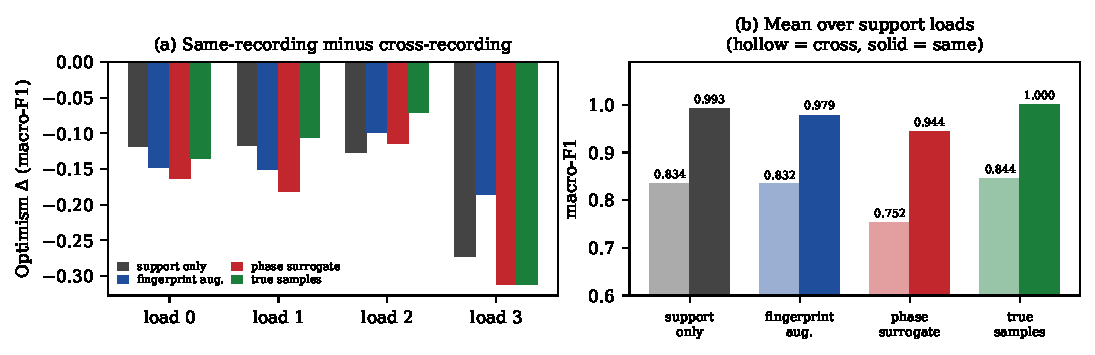
\includegraphics[width=0.98\textwidth]{figs/fig_leakage.pdf}
\caption{Same-recording versus cross-recording evaluation ($k=5$, three
seeds, two repetitions). (a)~The optimism $\Delta$ of each training configuration, per support
load: every bar is positive, i.e.\ every configuration looks better on its own
held-out windows than on other recordings, and the effect is largest exactly
where the literature's favourite direction (load~3) is involved.
(b)~Averaged over the four support loads. Hollow bars are cross-recording,
solid bars same-recording. No augmentation reliably beats training on the
labeled support set once the evaluation is cross-recording, and adding $400$
\emph{real} labeled samples per class ($0.844$) is within noise of the trivial
baseline ($0.834$).}
\label{fig:leak}
\end{figure}

\section{Cross-Benchmark Control: Paderborn}
\label{sec:paderborn}

CWRU cannot falsify the fingerprint explanation, because it does not contain the
control that would do so: every class has exactly \emph{one} specimen. We
therefore repeat the essential measurements on the Paderborn (KAt) dataset
\cite{lessmeier2016paderborn}, in which several independent bearings share each
damage class, measured under four operating conditions at 64\,kHz.

We use 21 bearings: 6 healthy (K001--K006), 9 artificially damaged (KA series)
and 6 damaged by accelerated lifetime tests (KI series). Classes are defined by
\emph{damage location}, read from the damage profile that ships with each
bearing (outer ring OR, inner ring IR, healthy) --- i.e.\ exactly the kinematic
distinction that a fault model can express. Windows are 4096 samples (64\,ms);
at 64\,kHz a 1024-sample window spans only 16\,ms, which is shorter than one
BPFO period at 1500\,rpm, and we find that all bearings then produce
indistinguishable spectra.

One caveat is recorded here rather than buried: in the subset we downloaded,
every KA bearing is outer-ring and every KI bearing is inner-ring, so damage
location and damage origin (artificial versus run-to-failure) are confounded.
This does not affect the finding below, where the result is the \emph{absence}
of any class-conditional spectral structure, but it would matter
for a claim about outer versus inner race specifically.

\subsection{Class-conditional spectra are a rig property, not a class property}

\begin{figure}[t]
\centering
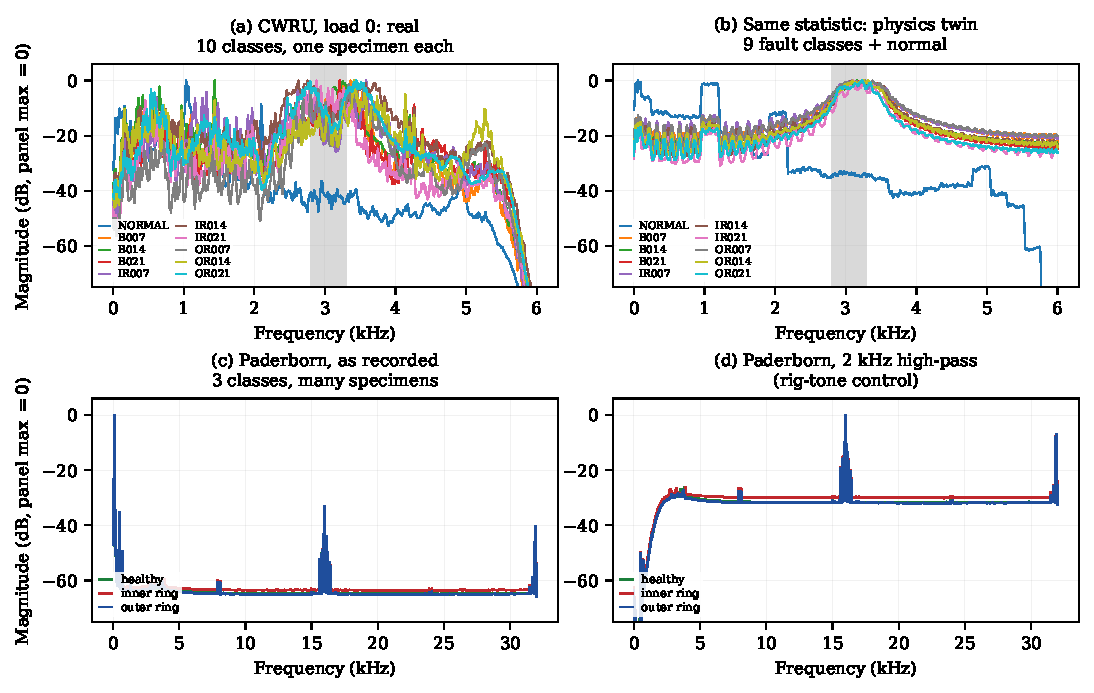
\includegraphics[width=0.98\textwidth]{figs/fig_spectra.pdf}
\caption{Class-mean magnitude spectra under the identical, unsmoothed
statistic of Table~\ref{tab:bench}. Each panel is normalized to its own maximum
(0\,dB); all four share the same $-75$\,dB floor, the same linear frequency
axis and the same per-class colours, and the shaded span marks the
$2800$--$3300$\,Hz band whose energy fraction is quoted in
Section~\ref{sec:diag2}. (a)~CWRU, ten classes, one physical specimen each:
visibly separated. (b)~The physics twin, same statistic: the nine fault classes collapse into one
band. Their median pairwise separation is $2.5$\,dB (minimum $0.9$\,dB), against
$6.7$\,dB (minimum $3.7$\,dB) for the nine real classes, and across frequency
the nine twin curves span a median of $6.5$\,dB against $18.8$\,dB. This is the
whole negative result in one panel --- the simulator produces nine faults whose
mean spectra are interchangeable, so no classifier trained on them can carry
the contrast that separates the real classes. (c)~Paderborn as recorded: the
$100$\,Hz rig line of Section~\ref{sec:paderborn} lands in the $93.75$\,Hz bin
(with leakage into its neighbour at $109$\,Hz) and carries essentially all the
energy, and the three damage
classes are indistinguishable because everything else lies $60$\,dB below it.
(d)~The same recordings after a $2$\,kHz high-pass removes that line --- the
objection that one dominant tone is flattening the comparison. The 16\,kHz rig
resonance now dominates, yet the three class means still track each other to
within a few dB across the whole band: the absence of class structure is not an
artefact of the tone. Compare (d) with (a), where the same statistic separates
the real classes by $10$--$30$\,dB.}
\label{fig:spectra}
\end{figure}

Table~\ref{tab:bench} compares the two benchmarks with one identical statistic:
the cosine similarity between class-mean magnitude spectra, shown directly in
Fig.~\ref{fig:spectra}.

\begin{table}[t]
\centering
\caption{Class-mean magnitude spectra, identical statistic on both benchmarks:
the \emph{unsmoothed} mean magnitude spectrum of each class, so the two
benchmarks are directly comparable. This is deliberately not the smoothed
envelope $A_c(f)$ of Section~\ref{sec:method} used elsewhere, which is smoother
and yields higher cosines.
``Within'' = different specimens, same class; ``between'' = different
specimens, different class. CWRU has one specimen per class, so only the
between-class numbers exist there; its ``same class across loads'' row is the
closest analogue of a within-class measurement. The last two rows remove the
rig tone of Section~\ref{sec:paderborn} by high-pass filtering at 2\,kHz,
which is the control for the objection that one dominant line could flatten
everything.}
\label{tab:bench}
\small
\begin{tabular}{llcc}
\toprule
Benchmark & Quantity & Cosine & Margin \\
\midrule
\multicolumn{4}{l}{\emph{CWRU (one specimen per class)}} \\
 & between class, load 0   & $0.626$ & --- \\
 & between class, load 3   & $0.626$ & --- \\
 & same class, load 0 vs 1 & $0.870$ & --- \\
\midrule
\multicolumn{4}{l}{\emph{Paderborn ($21$ specimens)}} \\
 & within class            & $1.000$ & \\
 & between class           & $1.000$ & $+0.000$ \\
\midrule
\multicolumn{4}{l}{\emph{Paderborn, high-pass $2$\,kHz}} \\
 & within class            & $0.992$ & \\
 & between class           & $0.989$ & $+0.003$ \\
\bottomrule
\end{tabular}
\end{table}

On CWRU the ten classes are strongly separated in the magnitude spectrum
(cosine $0.626$). On Paderborn, where a class contains several independently
manufactured bearings, averaging over specimens leaves \emph{no} separation at
all: within-class and between-class cosines are both $1.000$ to three decimals.
The spectra are dominated by a rig tone: at 1500\,rpm the largest spectral line
is at $100$\,Hz --- exactly four times the shaft rate --- in \emph{every one} of
the 21 bearings (measured on the full records it falls in $99.6$--$100.1$\,Hz
for all of them), healthy, outer-ring and inner-ring alike. In a
$4096$-point window that line lands in the bin at $93.75$\,Hz and
\emph{that single bin} carries $54\%$ of the total spectral energy
($53.97$--$54.31\%$ across the 21 bearings); the
line together with two neighbouring bins on each side carries
$99.5$--$99.8\%$.

That single tone invites an obvious objection to the claim above: of course the
class means coincide, if one line holds almost all the energy.
Filtering it away answers the objection. After high-pass filtering at
2\,kHz the within-class cosine falls to $0.992$ and the between-class cosine to
$0.989$; the margin moves from $0.000$ to $+0.003$. Removing the rig tone does
not reveal a hidden class signature --- there is none to reveal in the magnitude
spectrum --- which is the opposite of what happens on CWRU, where the
between-class cosine is $0.626$ in every load.

The two facts together identify the mechanism. The class separation that makes
CWRU look easy is not a property of the fault classes; it is a property of the
individual specimens and recordings that happen to carry the class labels. Where
several specimens share a label, the separation disappears.

\subsection{Same-recording leakage reproduces on a second benchmark}

If the optimism of Section~\ref{sec:protocol} were an artifact of CWRU, it would
not appear here. We train one model per seed on five bearings per class and
evaluate it twice: on held-out windows drawn from the \emph{same} bearings
($30\%$ of the training recordings), and on one bearing per class that the model
has never seen. Both test sets are class-balanced and the metric is macro-F1.
The two rows below are the two endpoints of
Table~\ref{tab:pb_levels}, and are taken from that same run.

\begin{table}[t]
\centering
\caption{Same-recording versus bearing-disjoint evaluation on Paderborn
(condition N15\_M07\_F10, three classes, 5 training bearings per class, 200
epochs, five seeds, macro-F1). The training set is files 1--4 of the training
bearings; the same-recording test set is its held-out $30\%$ of windows.}
\label{tab:pb_leak}
\small
\resizebox{\columnwidth}{!}{%
\begin{tabular}{lccc}
\toprule
 & Same recording & Bearing-disjoint & Optimism \\
\midrule
Mean over 5 seeds & $0.938$ & $0.597$ & $+0.340$ \\
Std. deviation    & $0.013$ & $0.139$ & \\
\midrule
\multicolumn{4}{l}{\emph{CWRU, for comparison} (mean over four support loads)} \\
Support only      & $0.993$ & $0.834$ & $+0.159$ \\
\bottomrule
\end{tabular}
}
\end{table}

The optimism is $+0.340$, well above the CWRU average and above CWRU's worst
case. Same-recording evaluation is not a quirk of one benchmark; it is a
consequence of drawing support and test windows from one recording, and it
reproduces wherever a benchmark is organized as a small number of long
recordings. We also note that under a bearing-disjoint protocol the features do
retain \emph{some} transferable signal ($0.597$ against $0.333$ chance) --- the
point is not that the task is unlearnable, but that more than half of the
apparent performance is leakage.

\subsection{The optimism decomposes into a session term and a specimen term}

The two endpoints above leave one thing unexplained, and it is the thing that
matters most for the interpretation: between them, \emph{two} factors change at
once. The bearing-disjoint test set is a different recording session \emph{and}
a different physical bearing. CWRU cannot separate them, because each class is a
single specimen. Paderborn can, because each of its 22 bearings was measured
$20$ times under the same condition: a model can be trained on files 1--4 of a
set of bearings and tested on files 5--8 of exactly those same bearings --- a
different recording session of the same specimen.

\begin{table}[t]
\centering
\caption{Decomposing the optimism. One training set (files 1--4 of five
bearings per class, first $70\%$ of windows) is evaluated on three test sets
that differ by exactly one factor each. Same condition, epochs and seeds as
Table~\ref{tab:pb_leak}; the L1 and L3 rows are that table's two columns.}
\label{tab:pb_levels}
\small
\resizebox{\columnwidth}{!}{%
\begin{tabular}{llcc}
\toprule
Test set & Changes from the level above & macro-F1 & Drop \\
\midrule
L1 same file, held-out windows & ---                       & $0.938$ & \\
L2 files 5--8, same bearings   & recording session only    & $0.755$ & $+0.182$ \\
L3 held-out bearings           & specimen as well          & $0.597$ & $+0.158$ \\
\bottomrule
\end{tabular}
}
\end{table}

The result is unambiguous and it splits the effect in two roughly equal parts.
Simply re-measuring the \emph{same} bearings costs $+0.182$ macro-F1: that much
of the optimism is pure session leakage, with the specimen held fixed. Changing
the specimen on top of that costs a further $+0.158$. Both terms are of the
same order, so the two explanations that the CWRU protocol cannot distinguish
--- ``the model keys on the recording'' and ``the model keys on the individual
bearing'' --- are in fact each about half right.

Two qualifications belong here. First, the specimen term is far more variable
than the session term: dropping it has a standard deviation of $0.139$ against
$0.032$ for the session drop, and one of five seeds (seed~3, $L3 = 0.82$) even
reverses the sign. Which bearing is held out matters more than which session it
was measured in, which is what one expects if the specimen term is carried by
that bearing's individual spectral signature. Second, $L3 = 0.597$ is above
chance, so cross-specimen transfer is not zero; it is roughly the level the
classes would reach from the fault \emph{physics} alone.

\subsection{Where the kinematics match the labels}

The Paderborn classes are defined by damage location, so here the impulse train
at BPFO/BPFI is not merely plausible: it is the right physics for the label. We
therefore repeat the no-source few-shot experiment of
Section~\ref{sec:results} with these classes, evaluating on held-out bearings.

\begin{table}[t]
\centering
\caption{No-source few-shot augmentation on Paderborn, classes defined by damage
location (healthy / inner ring / outer ring), bearing-disjoint test, macro-F1.
Chance is $0.333$. Five seeds at $k=5$, three at $k=20$ and $k=50$. The last
column is the same setting as
Table~\ref{tab:fewshot} except that the class labels are, on this benchmark,
consistent with the fault kinematics.}
\label{tab:pb_fewshot}
\small
\resizebox{\columnwidth}{!}{%
\begin{tabular}{lcccc}
\toprule
$k$ (windows/class) & Real support & Pure twin & Fingerprint & $+$ physics \\
\midrule
$5$  & $0.286$ & $0.166$ & $0.203$ & $0.199$ \\
$20$ & $0.316$ & $0.172$ & $0.177$ & $0.266$ \\
$50$ & $0.325$ & $0.166$ & $0.168$ & $0.231$ \\
\bottomrule
\end{tabular}
}
\end{table}

Three things are true in every row. Nothing beats simply training on the real
labeled samples. The pure twin is the \emph{worst} entry, below the chance level
of $0.333$, even though its physics matches the class definition exactly. And the
real-sample baseline does not improve with $k$ --- $0.286$ at five samples per
class, $0.325$ at fifty --- so the ceiling here is set by the bearing-disjoint
protocol, not by sample count. Within the augmentation columns the ordering is
stable too: layering the impulse train onto the target envelope is the highest
augmentation at $k=20$ ($0.266$ against $0.177$) and at $k=50$ ($0.231$ against
$0.168$), and is level with the envelope alone at $k=5$ ($0.199$ against
$0.203$). Both of those exceed the pure twin in all three rows.

We must be equally clear about what this table cannot do. With every entry at or
below chance, it cannot rank methods, and the differences between the
augmentation columns lie within one standard deviation. We report it for the
one comparison that is stable across all three values of $k$, and that is
externally corroborated.

\paragraph{A positive control for the mechanism.}
On CWRU, fingerprint calibration was the best augmentation and layering physics
on it consistently hurt. On Paderborn the ranking inverts: fingerprint
calibration alone is indistinguishable from the raw twin, and adding the
physical impulse train is what recovers the ground it lost. This is exactly
what the mechanism predicts. On CWRU the class information \emph{is} the
fingerprint, so estimating the fingerprint captures the label and physics is
redundant noise. On Paderborn we measured that the class-mean fingerprints are
identical across classes (margin $+0.003$, Table~\ref{tab:bench}); calibrating
to them therefore transfers no label information, and the only thing left
carrying the label is the impulse repetition rate --- the physics. The
methodological failure we diagnose is thus not a property of physics-based
augmentation as such, but of applying it to a benchmark whose class labels are
bound to individual recordings.

\section{Method: Target-Domain Spectral Envelope Calibration}
\label{sec:method}

Let $\{(\mathbf{x}_i,y_i)\}_{i=1}^{kC}$ be the labeled target support set for
$C$ classes. For class $c$ we estimate the magnitude envelope
\begin{equation}
A_c(f) \;=\; \frac{1}{|\mathcal{S}_c|}\sum_{i \in \mathcal{S}_c}
\bigl|\mathcal{F}\{ \mathbf{x}_i \odot \mathbf{w} \}(f)\bigr|,
\end{equation}
smoothed with a moving average of width $5$ bins and normalized to unit $\ell_2$
norm. Every envelope number quoted in this paper (hereafter the \emph{smoothed
envelope}) uses this definition; the unsmoothed class-mean spectra of
Table~\ref{tab:bench} are a different statistic and are not comparable to it.
Synthetic samples are then obtained by coloring an excitation $e$ in the
frequency domain,
\begin{equation}
\mathbf{x}_{\text{syn}} = \mathcal{F}^{-1}\bigl\{\, \mathcal{F}\{e\} \cdot A_c \,\bigr\},
\end{equation}
followed by per-window $z$-scoring. We consider two excitations: white noise
(the \emph{fingerprint} variant) and an impulse train placed at the
characteristic frequencies recomputed at the \emph{target} shaft speed
(the \emph{fingerprint$+$physics} variant).

Both variants use only the $k$ labeled support samples; no test window is
involved. The envelopes are accurate at small $k$: estimated from $k=5$
samples, the per-class envelope matches one estimated from the entire target
load at cosine $0.995$ on average ($0.989$ worst class). The corresponding
\emph{source-domain} envelopes match the target load only at $0.924$, which is
why the target-domain qualifier matters.

\section{Results}
\label{sec:results}

\subsection{Standard protocol}
Table~\ref{tab:main} reports the ten-class S0$\rightarrow$S3 comparison,
five seeds, all runs from a single uniform batch. Three observations.

\emph{The twin is worse than its own ablation.} Adding the calibrated physics
twin (\ml{dt\_dann}) reaches macro-F1 $0.914 \pm 0.078$, below plain adversarial
adaptation (\ml{dann}, $0.986 \pm 0.027$) and below the physics-free
augmentation ablation \ml{rand\_dann} ($0.922 \pm 0.098$). It is also the least
stable configuration.

\emph{The protocol saturates.} Every configuration that uses target labels
reaches $0.91$--$1.00$, leaving almost no headroom; the differences among
\ml{dann}, \ml{fp\_phys\_dann} and \ml{fp\_dann} are not a meaningful
demonstration of method quality in this regime. The informative comparisons are
in the constrained regimes of Section~\ref{sec:results}.

\emph{Performance is bounded by the labeled support set.} The zero-label bound
\ml{src\_pure} reaches $0.731$; merely adding the $k=5$ labeled target samples
(\ml{source\_only}) raises this to $0.823$.

\begin{table}[t]
\centering
\caption{Ten-class CWRU S0$\rightarrow$S3, $k=5$ labeled target samples per
class, five seeds, single uniform batch. \ml{src\_pure} uses no target data at
all; \ml{source\_only} and all remaining rows additionally use the labeled
support set.}
\label{tab:main}
\small
\resizebox{\columnwidth}{!}{%
\begin{tabular}{lcc}
\toprule
Method & Accuracy & macro-F1 \\
\midrule
\ml{src\_pure} (no target data)   & $0.8188 \pm 0.0421$ & $0.7307 \pm 0.0225$ \\
\ml{source\_only}                 & $0.8842 \pm 0.0377$ & $0.8228 \pm 0.0686$ \\
\ml{dann} (A2 ablation)           & $0.9904 \pm 0.0179$ & $0.9858 \pm 0.0268$ \\
\ml{rand\_dann} (A3 ablation)     & $0.9512 \pm 0.0553$ & $0.9223 \pm 0.0977$ \\
\ml{dt\_dann} (physics twin)      & $0.9028 \pm 0.1212$ & $0.9141 \pm 0.0780$ \\
\ml{fp\_phys\_dann} (fp.\ $+$ imp.)& $0.9917 \pm 0.0091$ & $0.9891 \pm 0.0123$ \\
\textbf{\ml{fp\_dann} (fp.\ $+$ noise)} & $\mathbf{0.9998 \pm 0.0003}$ & $\mathbf{0.9998 \pm 0.0004}$ \\
\bottomrule
\end{tabular}
}
\end{table}

\subsection{Constrained regimes}
The standard protocol saturates, so the meaningful comparisons are the
constrained ones. In the synthesis-only regime (Table~\ref{tab:synth}) the
physics twin is at chance ($0.123$) while fingerprint-coloured white noise
reaches $0.910$; adding the physical impulse train drops this to $0.651$, and
removing the fault-harmonic fine structure from the envelope drops it further
to $0.524$.

In the no-source regime, where only the $k$ labeled target samples are
available (Table~\ref{tab:fewshot}), the same ordering holds: the twin
augmentation is harmful at every $k$, whereas spectral augmentation
helps, and most at $k=1$ ($0.890 \rightarrow 0.977$). Source-domain
fingerprints, which need no target labels, remain clearly worse than
target-domain ones at every $k$ ($0.861$/$0.905$ against $0.977$/$0.993$).

\begin{table}[t]
\centering
\caption{No-source few-shot setting, target load~3, macro-F1. Each cell is $6$
runs (three seeds, the whole configuration repeated twice).
Augmentations add $400$ samples per class generated from the $k$ labeled
support samples only.}
\label{tab:fewshot}
\small
\begin{tabular}{lccc}
\toprule
Augmentation & $k=1$ & $k=3$ & $k=5$ \\
\midrule
none (support only)        & $0.890$ & $0.970$ & $0.985$ \\
physics twin               & $0.558$ & $0.777$ & $0.885$ \\
fingerprint $+$ white noise& $0.977$ & $0.995$ & $0.993$ \\
fingerprint $+$ impulse     & $0.947$ & $0.983$ & $0.658^{\dagger}$ \\
source fingerprint         & $0.861$ & $0.945$ & $0.905$ \\
phase surrogate            & $0.960$ & $0.993$ & $0.993$ \\
noise-only augmentation    & $0.952$ & $0.991$ & $0.994$ \\
true target samples (bound)& $1.000$ & $1.000$ & $1.000$ \\
\bottomrule
\end{tabular}
\\[2pt]
\footnotesize $^{\dagger}$ very high variance ($\pm 0.46$): two of six runs
collapse to $0.014$, well below the $0.10$ chance level. The sample is bimodal
rather than noisy.
\end{table}

\section{Discussion and Limitations}
\label{sec:discussion}

\paragraph{Scope.} The conclusion is emphatically \emph{not} that
simulation-based augmentation is useless in general. It is that the two
benchmarks we examine cannot test it, for different reasons that share a root.
On CWRU the class label is confounded with the recording, so the signal a
classifier learns is not the fault. On Paderborn the label \emph{is} physically
meaningful --- damage location, the very quantity whose characteristic
frequencies a model can compute --- yet the magnitude spectrum carries none of
it, because a single rig tone and its spectral leakage hold over $99\%$ of the
energy in every bearing whether healthy or damaged. A benchmark suitable for testing
physics-based augmentation must satisfy both conditions at once: the label must
have a physical definition, and the recording must actually expose it. Neither
of the two most-used public datasets does, and we suggest that establishing this
be part of benchmark validation rather than something each paper discovers
separately. The CWRU benchmark has already been criticised on related grounds
\cite{hendriks2022benchmark}; we add a mechanism and a quantitative control.
The situation is not unique to this field --- a model can generalise across
hospitals while relying on a site-specific confounder invisible in the
acquisition protocol \cite{zech2018variable} --- which is why we state the
requirement in terms of benchmark construction rather than of any one paper's
methodology.

This also reframes what the field should take from negative results. The
failure we diagnose is a property of the \emph{pairing} of a generator with a
benchmark, not of the generator. The same twin that is worthless on CWRU is, on
Paderborn, no longer the worst entry once its impulse train is layered onto the
target spectral envelope (Table~\ref{tab:pb_fewshot}): that is the only setting
in which we observe the physical component adding anything, and it is what the
mechanism predicts, since there the fingerprint carries no label and the only
remaining carrier of the label is the impulse repetition rate. The pure twin
remains the worst augmentation on \emph{both} benchmarks, and on neither does
any augmentation beat simply training on the real labeled support samples.

\paragraph{Implications for reported numbers.} Two papers reporting the same
method on CWRU may differ by $0.1$--$0.3$ macro-F1 purely because of how the
few-shot split was drawn. Future work should state whether support and test
come from the same recording, and ideally report both. The same control is
cheap wherever a dataset contains several independent specimens per class: hold
out specimens, not windows. Our own experience is a case in point. The
secondary tables in this paper are reported over six or twenty runs rather than
the conventional three, because repeated execution of \emph{the same command}
with the same seeds moved a ten-seed mean by up to $0.033$ and made a
three-seed standard deviation wrong by more than an order of magnitude. This is
the same problem that has been documented for reinforcement learning
\cite{henderson2018matters} and for evaluation budgets generally
\cite{dodge2019showyourwork}, and it argues for reporting score
\emph{distributions} and the compute spent on them.

\paragraph{A checklist for few-shot cross-domain results.} Concretely, we suggest
that a paper claiming few-shot cross-domain performance report, in addition to
its accuracy: (1)~whether support and test windows come from the same recording,
and the cross-recording number if they do; (2)~the same-recording number for a
trivial baseline that trains on the labeled support set alone, so that
augmentation gains can be read against it; (3)~the number of \emph{independent
specimens} per class in the target, which bounds what any augmentation can
transfer; (4)~for a simulation- or twin-based source, the shortest
characteristic period of the fault kinematics relative to the analysis window
(Paderborn at 64\,kHz fails a $1024$-point window on this alone); and (5)~the
class-mean spectra of the source and target domains, which is enough to detect
the fingerprint regime in which the label is bound to the recording. Items
(1)--(3) cost nothing beyond a second evaluation; item (5) is a single FFT per
class.

\paragraph{Limitations.} (i) We study two datasets and one backbone. (ii) The
cross-recording control on CWRU evaluates on a whole different load, which
confounds the recording change with the operating-condition change; a same-load,
different-session split is not available in CWRU, and we resort to Paderborn to
separate the two terms of Section~\ref{sec:paderborn}. There the separation
relies on $20$ repeated measurements per bearing, so it measures the session
term under one rig's repeat-measurement protocol and may not transfer to
datasets whose repeated recordings differ by more than a re-mount. (iii) Our
constructive method
is a regularizer rather than a uniform improvement, and we report it as such.
(iv) In the Paderborn subset we downloaded, every artificial-damage bearing is
outer-ring and every run-to-failure bearing is inner-ring, so damage location
and damage origin are confounded; our spectral claim is an \emph{absence} of
class structure and is unaffected, but it does not support a separate statement
about outer versus inner race. (v) The Paderborn few-shot entries all lie at or
below chance, so that table ranks nothing; we use it only for the two
comparisons that are stable across all three sample budgets. (vi) The spectral
comparison for Paderborn uses one operating condition and 21 bearings.

\section{Conclusion}
\label{sec:conclusion}

We showed that on CWRU cross-load bearing diagnosis the dominant class
information is a per-bearing recording fingerprint that physics cannot predict,
making simulation-based sample supplementation structurally ineffective; that
the standard few-shot protocol leaks this fingerprint from support to test and
inflates reported accuracy by $0.15$--$0.19$, rising to $0.31$ in the
hardest direction; and that a compact spectral envelope calibration estimated
from five labeled samples per class is the most robust augmentation available,
while adding physical impulse structure on top of it consistently hurts.

We then removed the objection that CWRU is simply a badly chosen dataset. On
Paderborn, where several independent bearings share each class, class-mean
magnitude spectra of healthy, inner-ring and outer-ring bearings are
indistinguishable (margin $+0.003$ after the rig tone is filtered out, against
$0.626$ on CWRU), so CWRU's class separation is a property of individual
specimens rather than of the classes; same-recording evaluation remains
optimistic, by $+0.340$, of which $+0.182$ is attributable to the recording
session alone and $+0.158$ to the change of specimen; and the physical component
of the twin becomes useful
for the first time once its impulse train is layered on the target envelope, in
the one setting where the labels rather than the fingerprints carry the physics
--- though the pure twin is still the worst augmentation there, and no
augmentation on either benchmark beats training on the real labeled support
samples. The practical recommendation is therefore not to abandon physics-based
generation, but to validate the benchmark before trusting either the positive or
the negative result obtained on it.

% >>> elsarticle-decl BEGIN(转换脚本插入,不是正文)
\section*{CRediT authorship contribution statement}
\textbf{Fangyu Zhang:} Conceptualization, Methodology, Software, Formal analysis,
Investigation, Resources, Writing -- original draft, Writing -- review \& editing,
Project administration.
\textbf{Julong He:} Supervision, Validation, Data curation, Visualization.

\section*{Declaration of competing interest}
The authors declare that they have no known competing financial interests or
personal relationships that could have appeared to influence the work reported
in this paper.

\section*{Funding}
This research did not receive any specific grant from funding agencies in the
public, commercial, or not-for-profit sectors.

\section*{Data availability}
The CWRU 12\,kHz drive-end and Paderborn KAt datasets analysed here are public.
The code and the per-table artifacts that reproduce every number in this paper
are provided as supplementary material to this submission.

\section*{Declaration of generative AI and AI-assisted technologies in the writing process}
During the preparation of this work the authors used ClawsGO Science Agent in
order to improve the language of the manuscript. After using this tool, the
authors reviewed and edited the content as needed and take full responsibility
for the content of the publication.

% <<< elsarticle-decl END

\bibliographystyle{elsarticle-num}
\bibliography{refs}

\end{document}
